\begin{document}
\thispagestyle{empty}
{\sans\fontsize{7.8}{10}\selectfont\color{muted}OUTSIDE-IN INVESTMENT MEMO \quad NOVEMBER 2026}\par
\vspace{2pt}
{\sans\bfseries\fontsize{19}{23}\selectfont\color{navy}Skello: what BDC V has to believe}\par
\vspace{1pt}
{\sans\fontsize{8.5}{11}\selectfont Pierre Grall, EDHEC Business School}\par
\vspace{3pt}
\note{Student case study from public sources only. I have no access to Skello or Bridgepoint data, and neither has seen this work. Reported figures carry a reference to the evidence ledger in the workbook (for example \src{E11}). Everything else is my estimate.}
\vspace{2pt}

\section*{Summary}
\textbf{From public sources alone, I cannot get the deal to my \V{hurdle_30} reference at about €350M post-money on ordinary shares.} Whether it gets there in reality depends on facts that only diligence can see. Base returns \V{base_moic} and \V{base_irr} at a December 2030 exit, against my reference of \V{hurdle_30} and \V{hurdle_irr}.\src{E19} The Downside returns \V{down_moic}. If the 2030 buyer is a sponsor underwriting a 15x EBITDA exit, Base falls to \V{base_nb} and the Downside to \V{down_nb}.

\textbf{Two answers would matter most in diligence: French gross retention, and the instrument.} Retention near \V{grr_25} with a 1x senior preference on the new money gives about \V{hurdle_25}, with the Downside at \V{down_pref} (\V{nb_pref} with a sponsor buyer). Neither is free: \V{grr_25} is above the \V{grr_cal} my calibration implies, and the preference would wipe out the rollover in the Downside, which sellers in an auction would resist.

\textbf{On price alone, \V{hurdle_25} would need a different deal.} It takes about €\V{pm_25}M post-money, below the €300--375M the press allows. At €150M that is a \V{pm_25_stake} stake and control; at the reported stake the cheque falls to about €\V{pm_25_cheque}M. A \V{irr_20} IRR takes €\V{pm_i20}M, \V{hurdle_irr} takes €\V{pm_i25}M and \V{hurdle_30} takes €\V{pm_30}M.

BDC V signed after a competitive process, with diligence I do not have.\src{E17} The gap measures what an outsider cannot see; it is not a verdict on the deal. Table 1 shows how far each unknown would have to move.

\begin{table}[H]
\caption{What closes part of the gap in Base, each taken alone}
\vspace{-2pt}
\tbl
\begin{tabularx}{\textwidth}{@{}P{3.1cm}LP{5.2cm}@{}}
\toprule
Unknown & What it takes & Result \\
\midrule
Retention above my \V{grr_base} & French gross retention of \V{grr_25}, with international and new logos moving with it & \V{hurdle_25}. \V{hurdle_30} would need \V{grr_30} \\
A protected instrument & 1x senior preference on the €200M of new money & Downside \V{down_moic} to \V{down_pref}. Base and Plan unchanged \\
A lower price than reported & Post-money of €\V{pm_25}M against the CFNEWS estimate of €350M\src{E11} & \V{hurdle_25}. See above on stake and range \\
A richer exit & \V{exit_adj_25} of revenue above my curve at exit & \V{hurdle_25}, at \V{exit_25_rev} of revenue in 2030 \\
\bottomrule
\end{tabularx}
\end{table}
\vspace{-5pt}

\begin{table}[H]
\caption{Three scenarios, exit December 2030, returns to Bridgepoint on ordinary shares}
\vspace{-2pt}
\tbl
\begin{tabularx}{\textwidth}{@{}L*{9}{R}@{}}
\toprule
 & ARR Dec-30 (€M) & Organic CAGR & EBITDA margin FY30 & Exit EV / revenue & Exit EV / ARR & Exit EV / EBITDA & MOIC & IRR & MOIC, sponsor buyer \\
\midrule
Downside & \V{down_arr30} & \V{down_cagr} & \V{down_margin} & \V{down_xrev} & \V{down_xarr} & \V{down_xebitda} & \textbf{\V{down_moic}} & \textbf{\V{down_irr}} & \V{down_nb} \\
Base & \V{base_arr30} & \V{base_cagr} & \V{base_margin} & \V{base_xrev} & \V{base_xarr} & \V{base_xebitda} & \textbf{\V{base_moic}} & \textbf{\V{base_irr}} & \V{base_nb} \\
Plan & \V{plan_arr30} & \V{plan_cagr} & \V{plan_margin} & \V{plan_xrev} & \V{plan_xarr} & \V{plan_xebitda} & \textbf{\V{plan_moic}} & \textbf{\V{plan_irr}} & \V{plan_nb} \\
\bottomrule
\end{tabularx}
\end{table}
\vspace{-6pt}

\begin{figure}[H]
\caption{Exit ARR and multiple needed for each MOIC}
\vspace{-3pt}
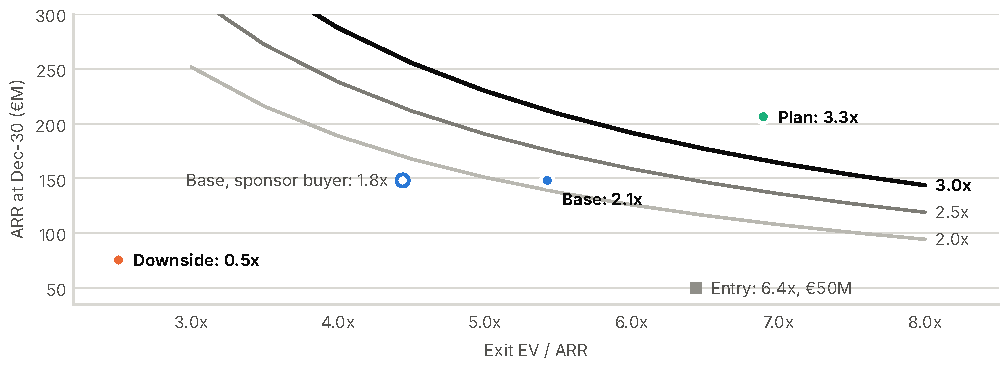
\includegraphics[width=\textwidth]{figures/required_arr.pdf}
\note{Lines use Base net debt and no new equity. Plan needs €\V{plan_follow}M of new equity, so it returns less than its position suggests.}
\vspace{-12pt}
\end{figure}

\section{The deal, rebuilt}
Reports give the cheques and the debt, plus a post-money that is CFNEWS's own estimate.\src{E08-E13} They do not split primary from secondary, so I assume €\V{primary}M of primary and €\V{existing}M of existing cash. Those two assumptions, not the press, produce the \V{m_entry} ARR.

\begin{table}[H]
\caption{Sources and uses at closing, and what they imply (€M)}
\vspace{-2pt}
\tbl
\begin{tabularx}{\textwidth}{@{}Lr@{\hspace{16pt}}Lr@{\hspace{16pt}}Lr@{}}
\toprule
\textbf{Sources} & & \textbf{Uses} & & \textbf{Implied} & \\
\midrule
Bridgepoint (BDC V) & \V{bp_eq} & Primary cash (assumed) & \V{primary} & Enterprise value & \V{ev_entry} \\
Founders and VCs, new money & \V{reinvest} & Purchase of existing shares & \V{secondary} & EV / ARR; EV / LTM revenue & \V{m_entry}; \V{ev_ltm} \\
Unitranche (Eurazeo) & \V{unitranche} & Costs and discount (assumed) & \V{costs_entry} & Bridgepoint stake & \V{bp_share} \\
\midrule
\textbf{Total} & \textbf{\V{sources}} & \textbf{Total} & \textbf{\V{sources}} & Cheque / BDC V (€2.8bn) & \V{ticket_fund} \\
\bottomrule
\end{tabularx}
\end{table}
\vspace{-3pt}

\textbf{Entry could be well away from \V{m_entry}.} Crossing post-money of €300--375M with primary of €20--100M gives \V{grid_low} to \V{grid_high} ARR and Base MOIC of \V{grid_moic_low} to \V{grid_moic_high}. Sources also disagree on whether the €200M includes the debt,\src{E10} but that changes only the secondary amount (€\V{secondary}M or €\V{secondary_b}M).

\begin{table}[H]
\caption{Price reference points, EV / revenue}
\vspace{-2pt}
\tbl
\begin{tabularx}{\textwidth}{@{}Lr@{\hspace{18pt}}Lr@{}}
\toprule
Skello at entry, on my assumptions & \V{ev_ltm} & Legacy time-and-attendance tools\src{E24} & 3--6x \\
My Rule of 40 curve at Skello's score & \V{curve_entry} & Scaled HCM suites\src{E24} & 5--8x \\
Band median, score 40--50\src{E23} & 7.0x & Paycor, 2025\src{E44} & \V{paycor} \\
Band median, score 30--40\src{E23} & 5.0x & Dayforce, 2025, growing 9.8\%\src{E25} & \V{dayforce} \\
\bottomrule
\end{tabularx}
\end{table}
\vspace{-3pt}

\textbf{On public data, the price sits at the top of the range.} Skello scores only \V{r40_gap} points above the drop from the 7.0x band to the 5.0x band. The bands are one adviser blog's blend of estimates, and I found nothing better in public. Growth of 40\% is the case for paying above tools and suites that trade lower.

\textbf{Two structural questions.} Pre-deal holders net €\V{selldown}M of cash, \V{selldown_pct} of their value, with Aglaé Ventures and the angels leaving,\src{E46} although management is reported to raise its stake.\src{E48} So debt and new equity fund a sell-down as well as growth. And €\V{cash_entry}M of cash beside a €40M loan costs about €\V{carry}M a year in negative carry, which suggests lower primary than I assume or cash held for build-ups.

\section{What the 2024 accounts show}
Skello's filed accounts for 2024 confirm the growth and change four assumptions.\src{E50-E57}

\begin{table}[H]
\caption{Skello SAS, statutory accounts (€M unless stated; French entity, Spain not consolidated)}
\vspace{-2pt}
\tbl
\begin{tabularx}{\textwidth}{@{}Lrr@{\hspace{22pt}}Lrr@{}}
\toprule
 & FY2023 & FY2024 & & FY2023 & FY2024 \\
\midrule
Revenue & \V{a_rev23} & \V{a_rev24} & Deferred revenue / revenue & \V{a_pca23} & \V{a_pca24} \\
Reported EBITDA & \V{a_eb23} & \V{a_eb24} & Cash at year-end & \V{a_cash23} & \V{a_cash24} \\
Reported EBITDA margin & \V{a_m23} & \V{a_m24} & Bank borrowings & \V{a_debt23} & \V{a_debt24} \\
Margin, development expensed & \V{a_x23} & \V{a_x24} & Average headcount & -- & \V{a_hc} \\
\bottomrule
\end{tabularx}
\end{table}
\vspace{-4pt}

\begin{itemize}
\item \textbf{Growth.} Revenue rose \V{a_growth} in 2024, in line with the 40\% reported.\src{E02}
\item \textbf{Profitability needs a definition.} The reported margin improved by \V{a_jump} points in a year, but €\V{a_capdev}M of development was capitalised in 2024, \V{a_capdev_pct} of revenue. My model expenses development, so the first question is on which basis 2025 was profitable.\src{E03}
\item \textbf{Customers pay ahead.} Deferred revenue is \V{a_pca24} of revenue and rose by \V{a_pca_inc} of the revenue increase. Growth releases cash, so I raised the working-capital inflow from \V{pre_nwc} to \V{new_nwc} of new ARR.
\item \textbf{Customer failures are visible.} Doubtful receivables equal \V{a_doubt} of revenue, and the 2024 bad-debt charge \V{a_bad}. This is the small-business closure risk behind the retention question, now in the accounts.
\item \textbf{Spain loses money.} Skello Iberia lost €\V{a_ib_loss}M on €\V{a_ib_rev}M of revenue, funded by €\V{a_ib_loan}M from the parent.\src{E55} International growth is the cash-hungry part of the plan.
\item \textbf{Other changes.} Tax credits were €\V{a_credit}M, so the research credit falls from \V{pre_cir} to \V{new_cir} of R\&D. Tax losses are about €\V{new_nol}M, not €\V{pre_nol}M, and existing net cash €\V{new_cash}M, not €\V{pre_cash}M. Together they move entry from \V{pre_m_entry} to \V{m_entry} ARR and leave Base MOIC at \V{base_moic2}.
\item \textbf{Shareholders.} Before the deal the founders held \V{a_founders} together, Partech \V{a_partech} and XAnge \V{a_xange},\src{E57} consistent with management near 40\% afterwards if the founders raised their stake.\src{E13,E48}
\end{itemize}

\section{What the public record cannot settle}
\subsection{Retention}
I reconstruct last-twelve-month revenue of about €\V{ltm_rev}M and net new ARR of €\V{net_new}M. Gross new ARR depends on sales spend and efficiency, and churn is what is left over. On my cost assumptions, S\&M above \V{sm_c} of revenue would mean a loss, which rules out part of the range.

\begin{table}[H]
\caption{Gross retention implied by public growth, at profitable levels of sales spend}
\vspace{-2pt}
\tbl
\begin{tabular}{@{}l*{3}{>{\raggedleft\arraybackslash}p{2.6cm}}@{}}
\toprule
S\&M share of revenue & CAC ratio \V{cac_a} & CAC ratio \V{cac_b} & CAC ratio \V{cac_c} \\
\midrule
\V{sm_a} & \V{g_a_a} & \V{g_a_b} & not feasible \\
\V{sm_b} & \V{g_b_a} & \V{g_b_b} & \V{g_b_c} \\
\V{sm_c} (break-even) & \V{g_c_a} & \V{g_c_b} & \V{g_c_c} \\
\bottomrule
\end{tabular}
\end{table}
\vspace{-3pt}

The public numbers still allow \V{grr_low} to \V{grr_high}. My calibration (\V{sm_cal} of revenue, CAC \V{cac_cal}) lands at \V{grr_cal}, and I use \V{grr_base} in France. A 38-client study puts SaaS at this contract size near 71\% and the next band near 81\%.\src{E30} It is thin evidence, so Table 6 runs down to that level. Core customers are small hospitality businesses, which close often.

\begin{table}[H]
\caption{Base MOIC by French retention and exit multiple. International moves with France; new logos adjust so last year's growth still ties}
\vspace{-2pt}
\tbl
\begin{tabular}{@{}l*{5}{>{\raggedleft\arraybackslash}p{2cm}}@{}}
\toprule
French gross retention & Curve \V{a0} revenue & Curve \V{a1} & Curve & Curve +\V{a3} & Curve +\V{a4} \\
\midrule
\V{l1} & \V{r10} & \V{r11} & \V{r12} & \V{r13} & \V{r14} \\
\V{l2} & \V{r20} & \V{r21} & \V{r22} & \V{r23} & \V{r24} \\
\V{l3} & \V{r30} & \V{r31} & \V{r32} & \V{r33} & \V{r34} \\
\V{l4} & \V{r40} & \V{r41} & \V{r42} & \V{r43} & \V{r44} \\
\V{l5} (Base) & \V{r50} & \V{r51} & \textbf{\V{r52}} & \V{r53} & \V{r54} \\
\V{l6} & \V{r60} & \V{r61} & \V{r62} & \V{r63} & \V{r64} \\
\V{l7} & \V{r70} & \V{r71} & \V{r72} & \V{r73} & \V{r74} \\
\bottomrule
\end{tabular}
\end{table}
\vspace{-3pt}

\subsection{Growth, history and market}
\begin{itemize}
\item \textbf{Run-rate.} Growth of 40\%,\src{E02} €40M at end-2025 and €50M today\src{E01} would imply \V{growth_h2} annualised in H2 2025 and \V{growth_h1} in H1 2026. Rounding could explain this: end-2025 at €42M removes most of the gap. A monthly ARR bridge settles it.
\item \textbf{History.} The 2021 plan announced 500 staff within two years and entry to Germany, Spain and Italy.\src{E31} Skello now has about 400 staff, and Germany is not among its listed countries.\src{E06,E32}
\item \textbf{Unit economics.} My calibration gives NRR of \V{nrr_fr} in France, payback of about \V{payback} months and LTV/CAC of \V{ltv_cac}. None is reported, and all depend on a CAC I fitted.
\item \textbf{Market.} French daily users are \V{pen_entry} of the 12M frontline workers the company cites,\src{E28} rising to \V{pen_base} in Base and \V{pen_plan} in Plan. They already equal \V{dau_hcr} of salaried hospitality staff,\src{E29} so growth depends on retail, health and other verticals.
\item \textbf{Competition.} Combo is about half Skello's size; Mapal and Toast cover restaurants; Factorial comes from payroll.\src{E47} Shiftbase, now sponsor-backed, is also aiming at Germany.\src{E40}
\end{itemize}

\section{Scenarios}
\begin{minipage}[t]{0.5\textwidth}
\vspace{0pt}
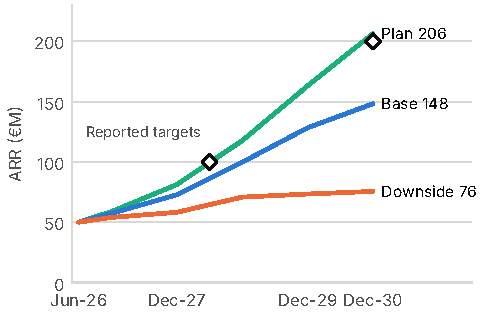
\includegraphics[width=\textwidth]{figures/arr_paths.pdf}
\end{minipage}\hfill
\begin{minipage}[t]{0.47\textwidth}
\setlength{\parskip}{4pt}
\vspace{2pt}
\textbf{Plan} follows the reported targets: €100M by 2028 and over €200M by 2030.\src{E14,E15} It needs \V{plan_cagr} organic CAGR.

\textbf{Base} takes \V{base_cagr} organic and €\V{base_acq_bought}M of bought ARR. It reaches €\V{base_arr28}M by end-2028, about six months behind the plan's date and with €10M bought.

\textbf{Downside} spends the money first: a build-up in FY28, R\&D that does not flex, French retention of \V{grr_down} and new-logo ARR down \V{down_new_drop} from the current rate.
\end{minipage}
\vspace{3pt}

\textbf{Exit.} EV is LTM revenue times a multiple read from the SaasRise bands, placed at their midpoints and joined by straight lines. Margin, CAC and retention therefore move the exit price, which a fixed ARR multiple would hide. Base scores \V{r40_base} on organic growth and gets \V{base_xrev}. The same score sits in a band whose median is 5.0x, where Base would return \V{base_band}.

\textbf{Spending and credit.} A large part of the proceeds is reported to go to AI,\src{E02} unquantified. Base carries €\V{ai_extra}M of R\&D above last year's share through FY29. A further €30M would cost \V{ai_cost} of MOIC, take FY27 EBITDA to about (€\V{ai_ebitda}M) and call €\V{ai_fo}M of new equity, which sits badly with reports that Skello stays profitable. Debt is \V{debt_arr} ARR, but \V{debt_ebitda} FY27 EBITDA. Cover is \V{cover_fy27} in FY27 in Base and \V{d_cover_27}, \V{d_cover_28} and \V{d_cover_29} over FY27--29 in the Downside, so only an ARR-style loan with liquidity tests fits. Terms are undisclosed, and I test no covenant.

\textbf{The preference.} In the Downside, €\V{down_dist}M is distributable, below the €200M preference, so the €\V{rollover}M rollover, most of management's stake, gets nothing. On Bridgepoint's cheque alone, the preference gives \V{pref_bp}. At illustrative weights of \V{w_d}/\V{w_b}/\V{w_p}, expected MOIC is \V{w_moic}, or \V{w_pref} with the preference, which is worth about the same as €\V{pref_cut}M off the post-money. With €20M of primary instead of €\V{primary}M, the Downside falls to \V{down_lowp} and calls €\V{down_lowp_fo}M of new equity.

\section{What moves the return}
\begin{minipage}[t]{0.5\textwidth}
\vspace{0pt}
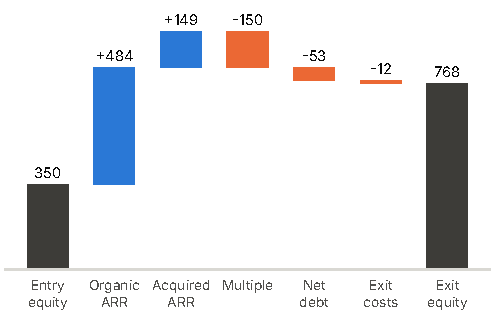
\includegraphics[width=\textwidth]{figures/bridge.pdf}
\end{minipage}\hfill
\begin{minipage}[t]{0.47\textwidth}
\setlength{\parskip}{4pt}
\vspace{2pt}
\textbf{Base equity value} goes from €350M to €\V{base_exit_eq}M (bridge at left, €M). ARR growth at the entry multiple adds €\V{br_arr}M, and the lower exit multiple takes back €\V{br_mult}M.

\textbf{Leverage barely matters.} With no debt at the same EV, IRR on total equity falls only from \V{lev_irr} to \V{unlev_irr}. In the Downside, debt lowers total-equity MOIC from \V{d_unlev} to \V{d_lev}.

\textbf{Holding longer adds MOIC.} Exit in 2029, 2030 or 2031 gives \V{moic_29}, \V{base_moic2} or \V{moic_31}, at \V{irr_29}, \V{base_irr} and \V{irr_31}, as margin and the multiple recover.
\end{minipage}
\vspace{1pt}

\begin{figure}[H]
\caption{One-at-a-time flexes on Base MOIC (exit multiple follows the Rule of 40 curve unless flexed directly)}
\vspace{-3pt}
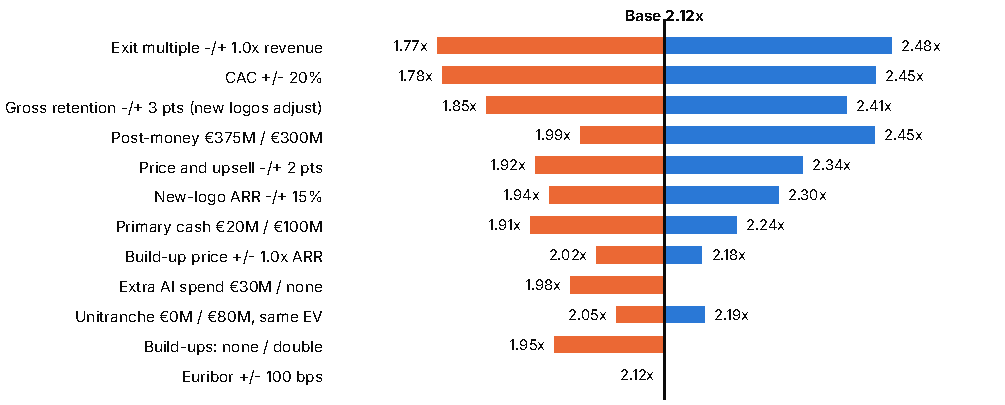
\includegraphics[width=\textwidth]{figures/tornado.pdf}
\vspace{-14pt}
\end{figure}

Three points of retention, 20\% on CAC and one turn of exit multiple each move MOIC by \V{tor_low} to \V{tor_high}; interest rates barely move it. Of the \V{gap_plan} between Base and Plan, organic ARR accounts for \V{step_org} and margins and CAC for \V{step_margin}, averaged over every order of the steps; build-ups take back \V{step_ma}.

\section{Exit: who pays \V{base_xrev} of revenue?}
Base exits at €\V{base_ev}M: \V{base_xrev} of revenue, \V{base_xarr} ARR and \V{base_xebitda} EBITDA on \V{base_org30} organic growth. Two yardsticks disagree on whether anyone pays that.

The curve reflects M\&A medians. LBO arithmetic shows what a sponsor can afford. Levering \V{nb_debt} EBITDA, reaching a \V{nb_cap} margin and earning \V{nb_irr}, it can pay €\V{nb_ev}M if it sells at \V{nb_exit} EBITDA in five years, which returns \V{base_nb} to Bridgepoint. At 13x or 17x it can pay €\V{nb_low_ev}M or €\V{nb_high_ev}M (\V{nb_low} or \V{nb_high}). If its own exit is priced on my curve, about \V{nb_curve_x} EBITDA, it can pay €\V{nb_curve}M. I weight 15x more heavily: it already sits above the \V{buyout_low}--\V{buyout_high} all-sector buyout median,\src{E45} and inside the 12--18x quoted for mature businesses.\src{E24} So €\V{base_ev}M needs either a strategic buyer, whose premiums are reported at 25--30\% over underlying multiples,\src{E24} or a sponsor who expects high multiples to last.

Strategics such as Xero, ELMO and Paychex have bought in this space, as have sponsors: Thoma Bravo directly, and Hg and TA through Access.\src{E25,E36,E37,E38,E44,E49} The Downside's \V{down_xrev} of revenue is \V{down_xebitda} EBITDA on \V{down_org30} growth, a price for the customer base. At 12x EBITDA it returns \V{down_12x}, or \V{down_12x_pref} with the preference. Whether Bridgepoint can force a sale from about \V{bp_share_short}, next to management at about 40\%, is a term I cannot see.

\section{Buy-and-build}
\textbf{Capacity covers a first step.} Cash above the minimum plus the capex line gives €\V{near_term}M, or about €\V{buy_5x}M of ARR at 5x after integration. Reports mention €5--20M of ARR per target and four or five targets.\src{E16} Cash generated to 2030 lifts capacity to €\V{capacity}M. At Base's organic rate, €200M of ARR needs €\V{plan_acq_at_base}M of acquired ARR and about €\V{plan_gap_at_base}M beyond capacity, falling to €\V{gap_30}M at 30\% organic growth. Debt at 4--5x FY30 EBITDA would add a net €\V{debt_low_net}--\V{debt_high_net}M, but that EBITDA arrives late. In equity, Bridgepoint's pro rata would take it to about €\V{exposure}M, or \V{exposure_pct} of the fund.

\textbf{Returns.} 5x plus \V{integration} of integration is \V{ma_eff} all-in against a \V{base_xarr} exit. Without build-ups Base returns \V{ma_none}, with them \V{base_moic2}. Doubling them lifts IRR to \V{ma_double_irr} and proceeds by €\V{ma_double_gain}M, but calls €\V{ma_double_fo}M of new equity and lowers MOIC to \V{ma_double}. I model no cross-sell, and the case for buying more depends on it.

\textbf{Recent deals.} Planday went to Xero,\src{E36} Rotaready to Access,\src{E38} Rotageek to ELMO,\src{E37} and Shiftbase to Fortino in April 2026.\src{E40} Eurazeo entered talks for Mapal, a hospitality suite, in 2025.\src{E39}

\begin{table}[H]
\caption{First-pass screen of what remains}
\vspace{-2pt}
\tbl
\begin{tabularx}{\textwidth}{@{}P{2.2cm}P{5cm}LL@{}}
\toprule
Target & What is known & Logic & Obstacle \\
\midrule
Combo (France) & 8,000 customer teams in 2024; €40M Series A led by Highland;\src{E42} half Skello's size\src{E27} & Closest French rival; per-employee pricing and payroll & Above the €5--20M range; price; competition review \\
Papershift (Germany) & Karlsruhe; several thousand customers in 10+ countries; Series A in 2021\src{E43} & Entry to Germany & Revenue undisclosed; may be small \\
Sesame HR (Spain) & \$23.2M FY25 revenue (CB Insights estimate); \$57.9M debt financing in 2025\src{E41} & Scale in Spain & Funded and likely a rival buyer \\
\bottomrule
\end{tabularx}
\end{table}
\vspace{-4pt}

\section{Diligence plan}
\begin{table}[H]
\vspace{-4pt}
\tbl
\begin{tabularx}{\textwidth}{@{}P{2.3cm}LP{6.4cm}@{}}
\toprule
Question & Data request & What the answer changes \\
\midrule
Retention & Euro and logo retention by cohort, country, sector and site count; closures split from competitive losses & About \V{grr_25}: \V{hurdle_25}. About \V{grr_20}: \V{hurdle_20}. Closures and competitive losses need different answers \\
Run-rate & Monthly ARR bridge from January 2025; price changes & If H1 2026 was mostly price, new logos are lower: 15\% fewer costs \V{newlogo_cost} \\
Sales efficiency & Fully loaded S\&M by country; payback by channel & CAC 20\% worse costs \V{cac_cost}, because margin moves the exit \\
International & Spain cohort P\&L after three years; Italy early data & \V{intl_share} of Base organic ARR growth rests on it \\
Earnings quality & Statutory accounts; capitalised development; research credit & Cash and tax losses settled by the 2024 accounts; open: capitalised development in 2025 profit \\
AI and pricing & Per-site against per-employee pricing; assistant usage and uplift; win/loss against AI-native entrants & One turn on the exit multiple moves MOIC by \V{exit_cost} \\
Build-ups & Target ARR, seller expectations, cross-sell evidence & Above about \V{base_xarr} all-in, a deal needs synergies \\
Structure & Instrument, drag-along, reserved matters; tax group and Charasse rule given founders roll over & Downside \V{down_moic} or \V{down_pref}, and whether Bridgepoint can force an exit \\
\bottomrule
\end{tabularx}
\end{table}
\vspace{-6pt}

\section*{Appendix}
\vspace{-6pt}
\begin{table}[H]
\caption{Base assumptions against the evidence}
\vspace{-2pt}
\tbl
\begin{tabularx}{\textwidth}{@{}P{4.1cm}P{2.5cm}L@{}}
\toprule
Assumption & Base & Basis \\
\midrule
Primary cash; existing net cash & €\V{primary}M; €\V{existing}M & Primary undisclosed. End-2024 cash €8.4M and bank debt €4.2M;\src{E52} near breakeven in 2025\src{E03} \\
French gross retention, FY27 & \V{grr_base} & Undisclosed. See Tables 6 and 7 \\
New-logo ARR, France / international, FY28 & €\V{new_fr_28}M / €\V{new_in_28}M & Set so organic growth slows from 40\%\src{E02} to \V{base_org30} in FY30 \\
CAC ratio, France / international, FY28 & \V{cac_fr_28} / \V{cac_in_28} & Calibrated: small LTM profit\src{E03} and implied headcount of \V{fte_ltm} against about 400\src{E06} \\
EBITDA margin, FY27 to FY30 & \V{margin_27} to \V{base_margin} & Follows from the lines above \\
Debt cost & \V{all_in} all-in & Euribor 2.32\%\src{E21} plus 6.50\%: top of the 5--6\% range plus part of the reported premium on AI-exposed software\src{E22} \\
Build-ups & 5.0x ARR, \V{integration} integration & Inside 3--6x;\src{E24} no cross-sell \\
Management incentive & \V{mip} above \V{mip_h} & Assumed. Management already holds about 40\%\src{E13} \\
Research credit & \V{new_cir} of R\&D & Tax credits of €0.15M in 2024.\src{E56} Counted as cash when earned \\
Reference return & \V{hurdle_30}, \V{hurdle_irr} gross & My assumption. Altaroc quotes BDC I--III at ``2.6 times net committed capital'' and 30\% IRR\src{E19} \\
\bottomrule
\end{tabularx}
\end{table}
\vspace{-5pt}

\begin{table}[H]
\caption{Where public sources disagree}
\vspace{-2pt}
\tbl
\begin{tabularx}{\textwidth}{@{}P{3.5cm}LP{5.1cm}@{}}
\toprule
Point & The disagreement & Treatment \\
\midrule
Bridgepoint's position & ``Lead minority shareholder'' in most reports; ``majority shareholder'' with 40--50\% in Consultancy.eu & Minority: \V{bp_share} on these figures \\
What the €200M contains & Equity plus separate debt (CFNEWS);\src{E08-E09} equity and debt together (Maddyness)\src{E10} & CFNEWS reading; returns unaffected \\
€100M ARR milestone & 2028 (Maddyness), 2027 (Veille de Presse), ``two years'' (CFNEWS)\src{E14-E15} & Mid-2028, as ARR \\
\bottomrule
\end{tabularx}
\end{table}
\vspace{-5pt}

\note{Model and checks: live-formula workbook with a separate Python implementation reconciled to it on \V{n_recon} values. That proves the file is consistent, not that its assumptions are right. Sources for every reported figure are in the workbook's Evidence tab.}
\end{document}
